\chapter{Reigniting non-mining investment} \label{chap2}

Point of this chapter

\begin{itemize}
    \item Show that investment and increases in capital stock is critical to income per capita growth and that it diverged since the GFC
    \item Demonstrate that australian non-mining investment has been flat since the peak of the mining boom
    \item Show that that is not due to compositional effects, but rather probably due to somewhat subdued demand, with interest rates supportive
    \item Note that in part the low i is not that low in real terms (inflation) and not that low comparatively, so still have relatively strong capital inflows, supporting the exchange rate and preventing very strong growth in trade exposed. This may be part of the `spread' of stagnation'.   
\end{itemize} 

\section{Australian investment experience since 2000 has been very different from rest of rich world}

Investment collapsed in the EU and US in 2008-9; no comeback in EU; comeback in US; contrasts with Australia (\Cref{fig:inv}).

\begin{figure}[p] 
 \caption{Investment dropped sharply in EU and US in 2008, not in Aust}
 \units{Gross capital formation (\% of GDP)}
 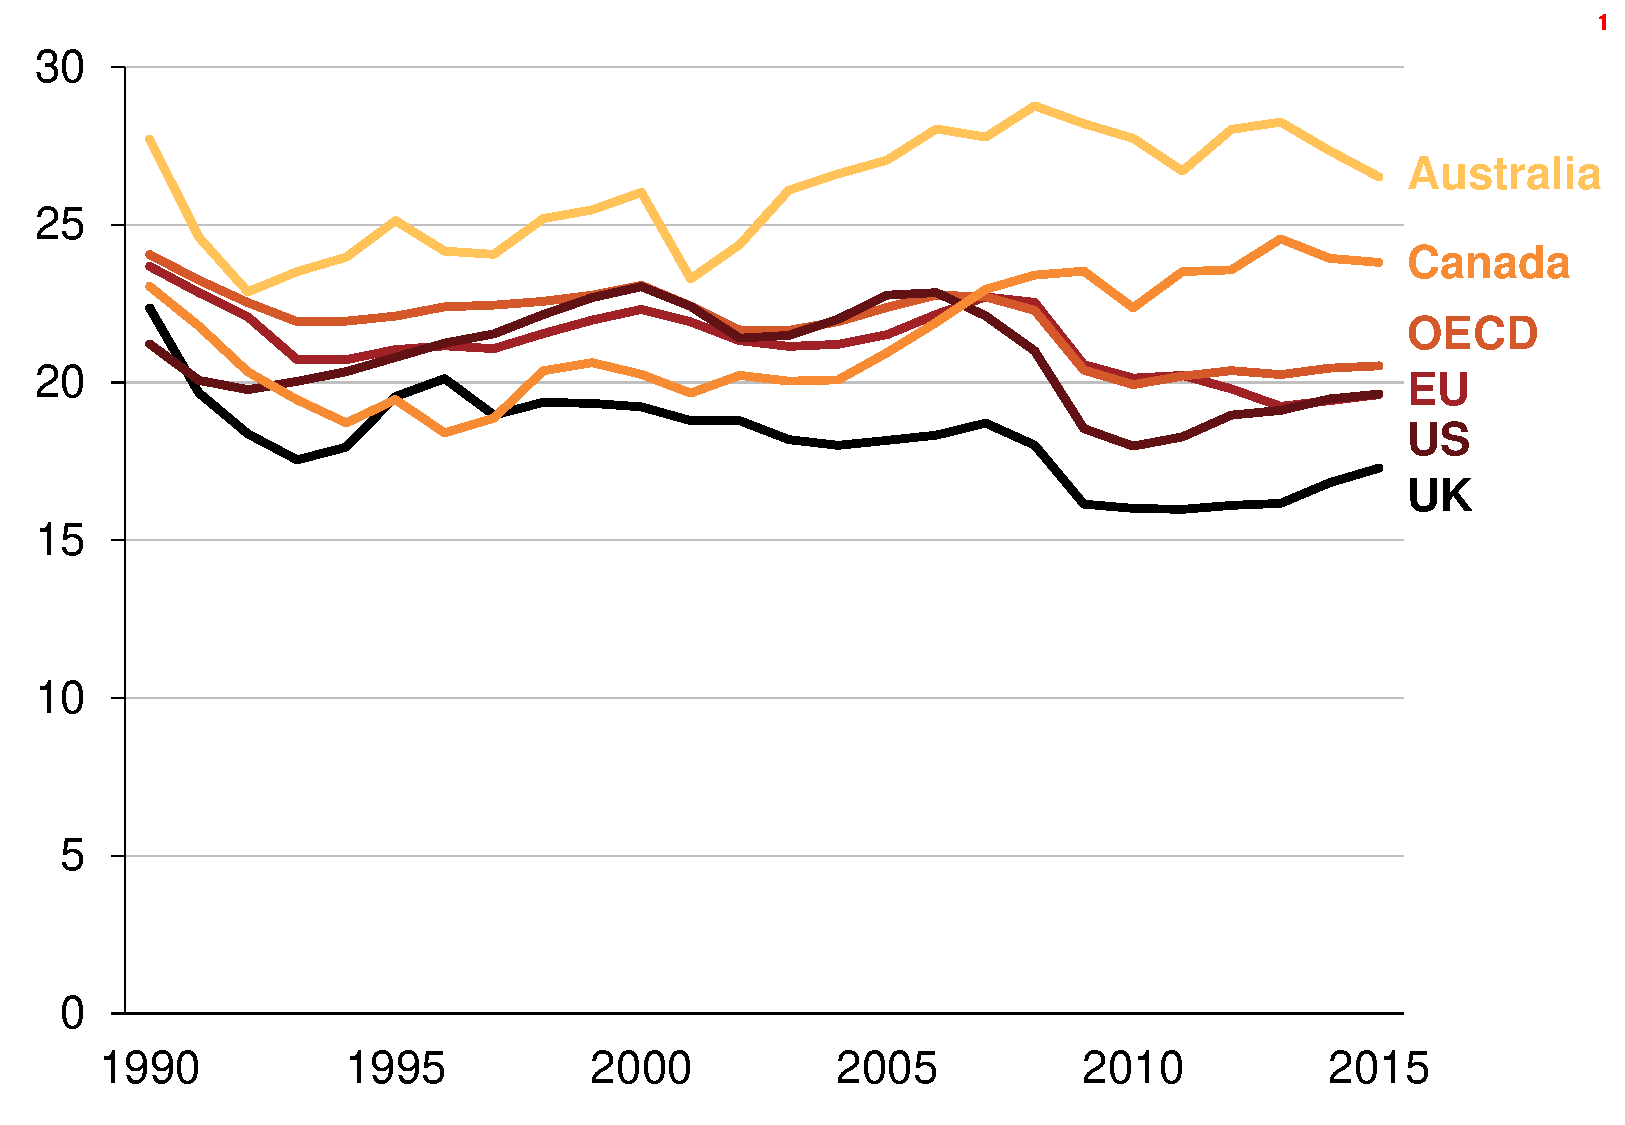
\includegraphics[page=1]{atlas/Ch2.pdf}\label{fig:inv}
\notes{GFCF including public investment and private dwellings}
\lucyi{look for EU, US, Aust private sector or at least non housing (investment per capita?? or per population of working age?? gets around the problem that cap per output or per work hour doesn't drop when output and hours drop too. Do Aust (mining) and Aust (non-mining?)}

\source{World Bank}
\end{figure}

\lucyi{This is all GFCF (inc dwellings and gov't) as \% of GDP, do you want to try chain volume measures?}

The collapse in EU and US gross investment matters a lot to the capital stock, because net investment fell much more. Eg in the EU and US the capital stock is about 2X GVA, and it decays at 6 per cent, so 12 per cent of GVA is needed just to keep cap:GVA constant). So net investment is much more variable than gross investment. And so the capital stock per capita also dropped off in the EU and US, but not in Australia -- even if you only look at non-mining capital (\Cref{fig:capstock}).\footnote{Probably need to have a footnote about different measures of the capital stock -- private vs total; including and excluding housing. It could be quite a long footnote if EU,US,AUS relativities vary depending on the metric but I doubt this.} 

\begin{figure}[p] 
 \caption{Cap stock per capita stagnated from 2008 in UK and US, Australia continued to grow strongly}
 \units{Capital stock in \$ US 2011 per capita}
 \includegraphics[page=2]{atlas/Ch2.pdf}\label{fig:capstock}
\notes{includes everything...(chain volume or constant price) in EU, US, Aust (total, prefer private sector or at least non housing capital stock per capita?? or per population of working age??. Could exclude mining}

\source{\textcite{feenstra2015}}
\lucyi{see alternatives: capital-output and capital per hour worked}
\end{figure}


\section{Australian investment has helped to drive incomes since 2000}

Investment is critical to output and income growth, because it maintains and increases the capital stock and embodies innovation.\footnote{Source.} Investment increases incomes by increasing the capital stock. \footnote{Rough estimate is if the return to K is say 40 per cent of GDP (which implies ROE of 20, which is too high, but anyway), then the elasticity of output WRT to capital is .4: a 10 percent increase in K:L increases output per worker by 4 per cent.} And investment embodies innovation -- because it is mostly done by firms that are growing faster because they have lower costs or better products. 

Need a chart???

US experience shows that low investment has reduced the capital stock per worker: labour market back near capacity but output per worker still down. \jim{'Potential output'} Australian output is probably X bigger than it would have been. Even non-mining investment. 

\lucyi{Partial source (for US) is in, or could be found in, Bob hall. }

% OECD definition of potential output is very different to Bob Hall's GDP shortfall. OECD potential seems to be an estimate of how far from the PPF given capital and labour participation rate. Need to discuss which concept to include.

\section{But Australian non-mining investment is yet to pick up}

\begin{figure}[p] 
 \caption{Private investment has been flat outside mining since 2007}
 \units{Private gross fixed capital formation as \% GDP}
 \includegraphics[page=3]{atlas/Ch2.pdf}\label{fig:privatecap}
\notes{Private gross fixed capital formation as a percentage of gross domestic product. GFCF excludes dwellings, transfer costs, and government and public corporations investment}

\source{ABS 5204.0 2014-15, Tables 52 (Private Gross Fixed Capital Formation, by Industry) and 5 (Gross Value Added by Industry)}
\end{figure}

\begin{figure}[p] 
 \caption{Private investment has returned strongly in non-mining states}
 \units{XXX}
 \includegraphics[page=4]{atlas/Ch2.pdf}\label{fig:statesinvestment}
\notes{***recreate chart once data source is confirmed*** RBA regards the error bars as material in this }

\source{ANZ Australia Insight August} 
\end{figure}

\begin{itemize}
    \item Private non-mining investment has fallen to recessionary 1990s levels
    \item But total private investment is still high and higher than it was at any point between 1990 and 2005
    \item Non-mining states are less anaemic. Non-mining investment in NSW continued to grow through the mining boom and both NSW and Victoria have picked up sharply in 2015. \footcite{RBA2016}
    \item Queensland and Western Australia are experiencing the post-mining boom transition most deeply and this is likely to continue in the short term.
    \item but compared to others Australian capital stocks look very health and continued to grow as others stagnated due to low investment barely meeting depreciation rates
\end{itemize} 

\begin{figure}[p] 
 \caption{Growth in nominal non-mining investment has been weak since the GFC}
 \units{Annual change in nominal GFCF, 1990-2015, percentage}
 \includegraphics[page=5]{atlas/Ch2.pdf}\label{fig:growcap}
\notes{Excludes mining, dwellings, transfer costs, and government and public corporations GFCF}

\source{ABS 5204.0 T52 Private Gross Fixed Capital Formation, by Industry - Current prices
}
\end{figure}

\section{The flatness of non-mining investment seems to be due to weak demand}

\begin{itemize}
    \item Growth in non-mining output has averaged only 3 per cent since 2012 after 20 years averaging 6 per cent annual growth.
    \item Net migration has declined 40 per cent (check) so low labour force participation growth, also baby-boomer retirements
    \item Capital stocks are high after strong non-mining investment through the 2000s
    \item And low demand
\end{itemize}

\begin{figure}[p] 
 \caption{Weak demand is driving low non-mining investment}
 \units{Annual change in nominal non-mining GDP, 1990-2015, percentage}
 \includegraphics[page=6]{atlas/Ch2.pdf}\label{fig:gdpgrowth}
\notes{Excludes mining. ***check for other exclusions***}

\source{ABS 5204.0 T5 Gross Value Added (GVA) by Industry
}
\end{figure}

\begin{figure}[p] 
 \caption{Business lending rates have been accommodative}
 \units{Nominal bank lending to business rate, percentage}
 \includegraphics[page=7]{atlas/Ch2.pdf}\label{fig:businessrate}
\notes{Excludes mining. ***find real business lending rates***}

\source{RBA, Bank Lending to Business – Selected Statistics – D8
}
\end{figure}

In recent years, wages have risen slowly, whereas capital goods prices have risen quickly. Both factors create further headwinds for short-term investment decisions.

Wage price growth is now low after many years of strong wage price growth up to 2014. Relatively cheap capital goods during the mining boom may have brought forward some investment. Capital goods prices were flat for nearly 4 years between 2009 and 2013 but have increased since (check). This is in part due to the falling exchange rate making imported capital goods more expensive.

Unless these changes are considered permanent shifts in the relative growth rates of capital and labour prices it would not be anticipated to have long-term effects on the investment rate. 

\section{Capital-output ratio and age of capital stock not too bad}

\begin{figure}[p] 
 \caption{Capital intensity for non-mining has been steady}
 \units{Non-mining capital-output ratio}
 \includegraphics[page=8]{atlas/Ch2.pdf}\label{fig:capout}
\notes{Excludes mining. ***check other exclusions***}

\source{ABS 5204.0 Table 5. Gross Value Added (GVA) by Industry, Table 63. Net Capital Stock, by Industry by type of asset
}
\end{figure}

The decline in non-mining capital intensity through the 1990s was predominantly due to a decline in capital intensity in capital light industries. Capital light industries, such as construction, financial and insurance services, and hospitality services, have reduced their capital intensity by up to 60 per cent since 1990. \footnote{Some of the decline in capital light industries is offset by capital-output increases in other sectors. Capital-heavy sectors have tended to increase their intensity, some of which is a one-off increase (mining and utilities), and some of which is the result of capital light sectors moving to renting their capital (buildings and equipment).}

A shift towards service sectors would be expected to lower the capital-output ratio as service sectors and construction tend to have low capital to output ratios. But this has only had a small impact compared to the decrease in intra-industry capital intensity.

Non-mining capital intensity has been relatively stable since the early 2000s. \footnote{The UK and US experienced a sharp increase in capital intensity through the GFC due to the sharp decline in output. Low investment and increasing output have resulted in a steady decline in their capital-output ratio since 2009.}

\begin{figure}[p] 
 \caption{Sectoral change has had minimal impact on the capital output ratio}
 \units{Percentage change in capital output ratio by cause}
 \includegraphics[page=9]{atlas/Ch2.pdf}\label{fig:sectorshift}
\notes{Excludes mining. *6 year period ***check other exclusions***}

\source{Grattan analysis of ABS 5204.0 Table 58 Capital Stock by Industry, 2014-15, and 5206.0 Table 6 Gross Value Added by Industry, 2016
}
\end{figure}

\section{What to do}

Macro environment

Regulation

Public investment - infrastructure

% Ampersand (&) must not be used unescaped (use \& instead)) - HP
Taxes \&\ industry assistance - corporate tax rate, R\&D support, depreciation rate, green investments

Tax rates?

Public vs private
(reft to https://www.pm.gov.au/media/2016-08-17/ceda-keynote-address-melbourne) 


\chapter{The precarious precipice: low investment as a main bit of secular stagnation} \label{chap_a}

\section{Global secular stagnation risk}

Chart: TFP since 1950

\section{Global slow output/investment/wages/everything}

 Chart:Output per capita - 2015 exchange rates

\section{Why do we care about investment?}

Chart: Capital-output ratio, international?

\begin{smallbox}{Investment in Growth Theory}{box:growth_theory}
\end{smallbox}

\chapter{It's not so bad: Australian investment in a global context} \label{chap_b}

\section{History of investment in Australia}

Chart: Investment % of GDP, inc forecast to 2017

\section{Global developed world falls in investment, Australian comparison}

Chart: global comparisons of investment % of GDP

\section{The steadiness of foreign investment in Australia}
q: bring up broader k stock before doing foreign share
need to show how important foreign investment has long been to investment in australia

Chart: foreign investment ABS 5352.0

\section{Bits and pieces}

Chart: dwellings didn't suck up investment (Dwellings investment \% GDP pretty steady)

Chart: Captial stock per capita


\chapter{Actually, it's not great: non-mining states are ``European''} \label{chap_c}

\section{Mining states and non-mining states took contrary paths}

Mining states increased investment well in excess of historical averages compared to non-mining states. 

Crowding out non-mining states investment?

Chart:mining vs non-mining states

\section{Non-mining states took a path similar to the rest of the world}
Non-mining states stagnated during the mining boom, their investment path was similar to US/EU losing about 3 percentage points of investment to GSP/GDP.

Chart: Total GFCF to GSP/GDP (including EU/US?)

\lucyi{do we want to look at any other state based differences, like wages, employment etc that support the overall story?}


\chapter{Accept the things we cannot change: medium term drivers of investment} \label{chap_d}

\section{Demand}

Chart: GDP growth (convert to real) and real change in private business GFCF

\section{Macro settings}

Interest rates are accommodative, real business lending rates have fallen. RBA has had a solid track record and room to move.

Hurdle rates inhibiting investment?

Chart: business lending rates
Chart: business lending to business investment ratio

\section{Cost of capital goods}

Chart: Capital goods price index

\section{The economy has not yet shifted to capital-light service sectors}

Overall: small shift to capital light sectors
Sectoral (while some cap-intense sectors shrank as share of economy eg manu, x, y; others grew eg utilities).

Any evidence about whether other high-income economies or leading companies are much more capital light, suggesting we might head more in that direction. Eg - is there a fact base in any of the discussion about secular stagnation that ties low investment demand to 'technology / structural' shifts in capital intensity. 

Chart: capital intensity chart combined with sectoral shift and intra-industry decline in intensity \% change

\begin{smallbox}
{Other than mining, service sectors growing}{box:sectors}
\end{smallbox}

\section{Uncertainty is worse than corporate taxes}

Can we show uncertainty? Ideally a chart. 


\chapter{So what then...} \label{chap_e}
\section{Company tax cuts}
Whether they be good or bad it won't fix the "hole" in investment.

Logic: with dividend imputation, C tax has little impact on investment by australian investors. ? about tax treaties ? but probably some impact on investment by offshore entities. (Though how big when there is massive profit shifting). 

Not necessarily a great time to do it. 

Quality of evidence is not very strong. Big error bars.

Chart showing investment (or capital: output ratio) vs tax rate by country. 

Other aspects of tax treatment eg depreciation?

\begin{smallbox}{The jury is out on company tax cuts}{box:corporate_tax}

\begin{itemize}
% For a list item with an empty symbol/bullet, use \item[]. 
    \item[] The bad
    \item Janine Dixon: would cost \$1600 pp
    % You can use \url for URLs.
    \url{https://www.vu.edu.au/news-events/news/company-tax-cut-not-in-national-interest}
    \item It's just a hand out to foreign investors
    
    The good
    \item Alternative modelling shows a positive impact on GNI after 10 years \url{https://grattan.edu.au/news/the-full-story-on-company-tax-cuts-and-your-hip-pocket/}
    \item It's largely a hand out to foreign investors, but Australians still benefit
    
    Issues
    \item Dividend imputation makes Australia different to others
    \item Australia's tax rate hasn't inhibited investment in the past, have global corporate taxes fallen recently and sufficiently to increase the need for a corporate tax cut?
    
    Overall
    \item A 1\% boost to GDP in 20 years is not a solution to a short term 2-3 percentage point decline in investment (as \% of GDP)
    \item Targeted policy (short term?) for investment may be a better alternative
    
\end{itemize}
\end{smallbox}

\section{Regulatory burden}

Evidence on the regulatory burden says...
X- country?? 'WEF' indices
(also they have them on innovation-friendliness which might be useful to split out)

Possible evidence on 'red tape reduction'? 

Zoning? 

\section{Invest in growth supporting public infrastructure}

Better targeted infrastructure will be conducive to growth by by itself will not fill the "hole"

still no reason to build bad stuff. in fact main argument should be that we are building the wrong stuff. building the right stuff is best. 
 
 \section{Complementary inputs: skilled labour}
 
 Immigration and education policies will influence future demand for capital. 
 
 Have we got the balance right? 
 
 \section{pro-competition and financial structure?}

eg industry super ...
eg excessive housing investment?


 \section{what do the business groups ask for?}
 ??

 
\begin{smallbox}{Free trade agreements}{box:fta}
\end{smallbox}

\begin{smallbox}
{Green investment - two birds one stone}{box:green_investment}
\end{smallbox}